\chapter{Cloud Security with Honeypots}

\section{Introduction}

%\todo{Daten sammeln mit T-Pot fuer Auswertungen, etc.. Bezug auf bisherige Arbeiten nehmen}

As previously mention in \fullref{sec:cloud-computing}, using cloud resources are becoming the go-to option for new services.
\citet{Kelly2021} investigated thoroughly cloud providers such as Azure, AWS, or Goolge Cloud. 

% \citet{Nithin2012}

\section{HeiCloud}

\citet{urz2021} offers a \enquote{\ac{iaas} specially tailored for higher education and research institutions}.
It supplies multiple institutes at University Heidelberg.
In addition, HeiCLOUD is a with DFN 

As stated on their information site, it offers the following features \cite{heicloud2021}:

\begin{itemize}
    \item IaaS for science:
    \item Freely manage IT resources by yourself:
    \item Stable and fast connection:
    \item High availability:
    \item High security standards:
    \item High scalability:
    \item Open Source:
    \item Freely selectable VM operating systems:
    \item Transparent accounting:
    \item Available in the German Research Network:
\end{itemize}

\textbf{OpenStack}

Besides several cyber security , honeypots are 

\section{T-Pot}

T-Pot is a hollistic approach to capture recent cyber attacks by the sheer quantity of various honeypots.
The German IT provider Telekom  
In conjucntion with a \\

\textbf{ADBHoney} \cite{adbhoney2021} is a low interaction \ac{adb} honeypot over TCP/IP.
The importance of this honeypot lies in the \ac{adb} protocol that is used to debug and push content to the device.
However, unlike USB it does not support any kind of ample mechanisms of authentication and protection.
By exposing the \ac{adb} service over any port, any adversary could connect and exploit this device.
ADBHoney is designed to catch malware that has been pushed onto the device.\\

\textbf{Cisco \ac{asa}} \cite{cymmetria2018} is a low interaction honeypot that detects CVE-2018-0101.
It is a vulnerability that could allow an unauthenticated, remote attacker to cause a reload of the affected system or to remotely execute code.
By sending multiple, crafted XML packets to a  \\

\textbf{citrixhoneypot} \cite{citrixhoneypot2020}\\

\textbf{conpot} \cite{conpot2021}\\

\textbf{cowrie} \cite{cowire2021}\\

\textbf{ddospot} \cite{ddosspot2021}\\

\textbf{dicompot} \cite{dicompot2021}\\

\textbf{dionaea} \cite{dionaea2021}\\

\textbf{elasticpot} \cite{elasticpot2021}\\

\textbf{endlessh} \cite{endlessh2021}\\

\textbf{glutton} \cite{glutton2021}\\

\textbf{heralding} \cite{heralding2021}\\

\textbf{hellpot} \cite{hellpot2021}\\

\textbf{honeypy} \cite{honeysap2021}\\

\textbf{honeysap} \cite{honeysap2021}\\

\textbf{honeytrap} \cite{honeytrap2021}\\

\textbf{ipphoney} \cite{ipphoney2021}\\

\textbf{mailoney} \\

\textbf{medpot} \cite{medpot2021}\\

\textbf{rdpy} \cite{rdpy2021}\\

\textbf{redishoneypot} \\

\textbf{snare} \cite{snare2021}\\

\textbf{tanner} \cite{tanner2021}\\


\begin{table}[h]
    \centering
    \caption{Overview of all available honeypots of T-Pot}
    \begin{tabularx}{\linewidth}{l|l|l}
        \toprule
        \textbf{Honeypot}                                 & \textbf{Description} & \textbf{Port} \\
        \hline
        adbhoney                                 &             &      \\
        ciscoasa \cite{cymmetria2018}            &             &      \\
        citrixhoneypot \cite{citrixhoneypot2020} &             &      \\
        conpot \cite{conpot2021}                 &             &      \\
        cowrie \cite{cowire2021}                 &             &      \\
        ddospot \cite{ddosspot2021}              &             &      \\
        dicompot \cite{dicompot2021}             &             &      \\
        dionaea \cite{dionaea2021}               &             &      \\
        elasticpot \cite{elasticpot2021}         &             &      \\
        endlessh \cite{endlessh2021}             &             &      \\
        glutton \cite{glutton2021}               &             &      \\
        heralding \cite{heralding2021}           &             &      \\
        hellpot \cite{hellpot2021}               &             &      \\
        honeypy \cite{honeysap2021}              &             &      \\
        honeysap \cite{honeysap2021}             &             &      \\
        honeytrap \cite{honeytrap2021}           &             &      \\
        ipphoney \cite{ipphoney2021}             &             &      \\
        mailoney                                 &             &      \\
        medpot \cite{medpot2021}                 &             &      \\
        rdpy \cite{rdpy2021}                     &             &      \\
        redishoneypot                            &             &      \\
        snare \cite{snare2021}                   &             &      \\
        tanner \cite{tanner2021}                 &             &      \\
        \bottomrule
    \end{tabularx}
    \label{tab:overview-honeypots}
\end{table}

In addition, T-Pot integrates following tools to investigate and handle network traffic:

\begin{itemize}
    \item Cockpit
    \item Cyberchef
    \item ELK stack
    \item Elasticsearch head
    \item Fatt
    \item Spiderfoot
    \item Suricata
\end{itemize}

\todo{Erstelle eigene uebersicht}
\begin{sidewaysfigure}[h]
    \centering
    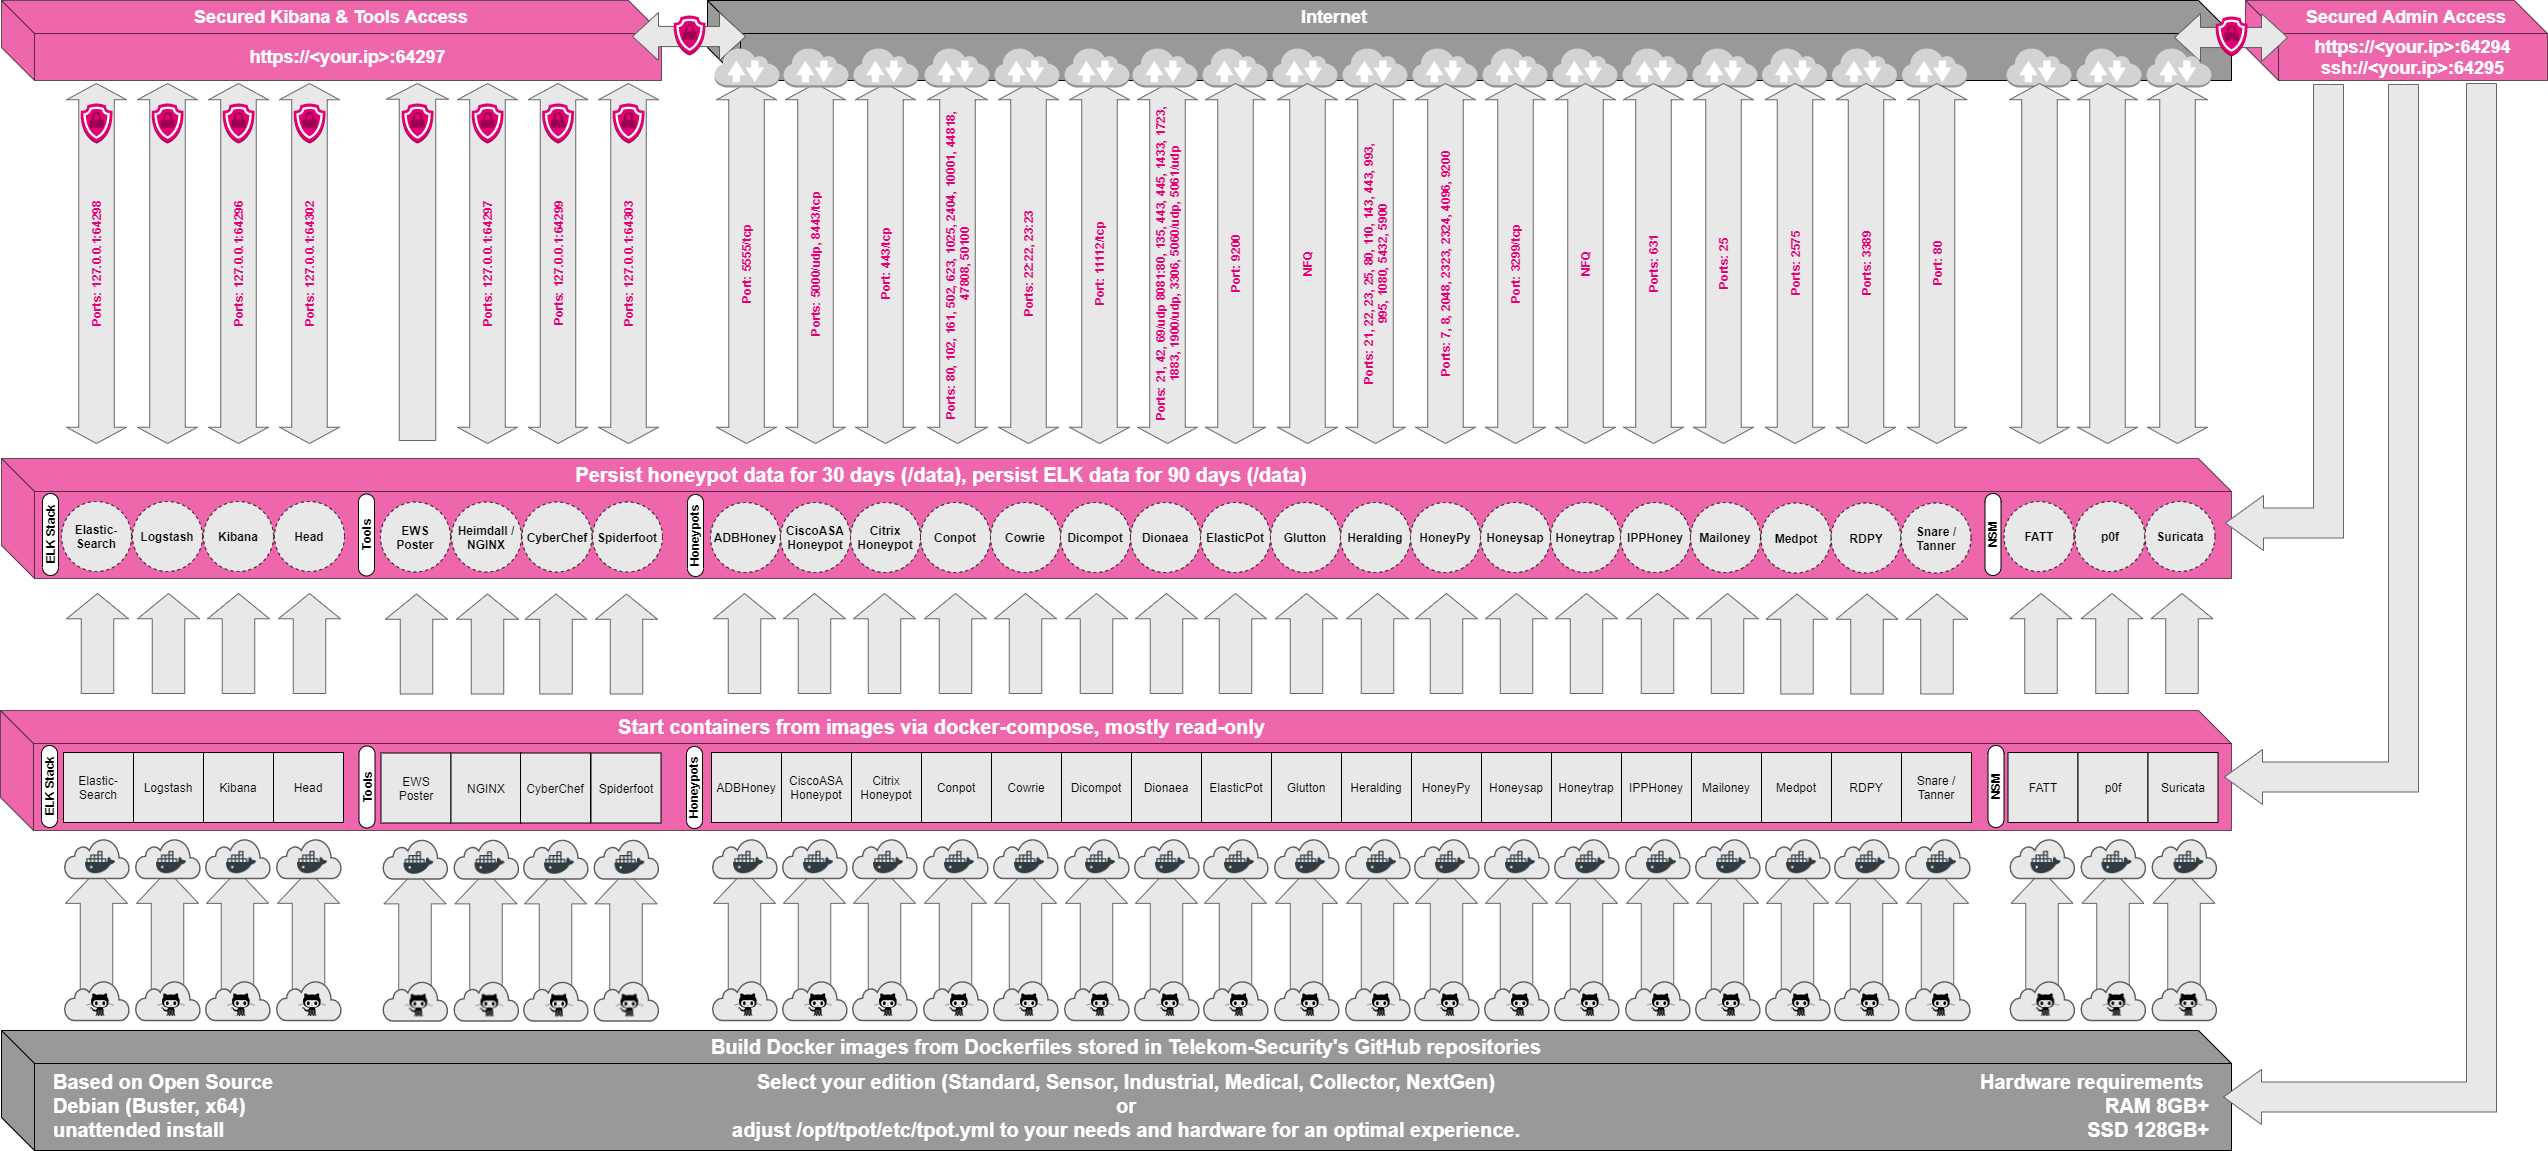
\includegraphics[width=\textwidth]{figures/architecture.png}
    \caption{}
    \label{fig:overview-tpot}
\end{sidewaysfigure}

\section{Data Analysis}

\citet{NawrockiWSKS2016} have done a sophisticated survey of honeypots and data analysis.
Based on their findings we give a short summary of the honeypot data analysis.

\begin{enumerate}
    \item Attack Profile
    \item Attack Source
    \item Attack Target
    \item Attack Frequency
    \item Attack Evolution
    \item Propagation of Attacks
    \item Attack Patterns
    \item Attack Root Cause Identification
    \item Attack Risk Assessment
    \item Exploit Detection
\end{enumerate}

\todo{übersicht tabelle}
\begin{table}[h]
    \centering
    \caption{}
    \begin{tabularx}{\linewidth}{l}
        \toprule
        Attack Profile\\
        Attack Source\\
        Attack Target\\
        Attack Frequency\\
        Attack Evolution\\
        Propagation of Attacks\\
        Attack Patterns\\
        Attack Root Cause Identification\\
        Attack Risk Assessment\\
        Exploit Detection\\
        \bottomrule
    \end{tabularx}
    \label{tab:overview-data-analysis}
\end{table}


\section{Results in HeiCloud}

\todo{verwendung von Grafiken, etc.}

\todo{show results}

Despite the amount of honeypots, we restrict ourself to consider only a few honeypots.
Reason for that is the \fullref{chap:concept}

\section{Summary}

In this chapter we have 